% This is samplepaper.tex, a sample chapter demonstrating the
% LLNCS macro package for Springer Computer Science proceedings;
% Version 2.21 of 2022/01/12
%
\documentclass[runningheads]{llncs}
%
\usepackage[T1]{fontenc}
% T1 fonts will be used to generate the final print and online PDFs,
% so please use T1 fonts in your manuscript whenever possible.
% Other font encondings may result in incorrect characters.
%
\usepackage{graphicx}
\usepackage{amsmath}
\usepackage{amssymb}
\usepackage{bm}
\usepackage{booktabs}
\usepackage{multirow}
\usepackage{subcaption}
\usepackage{placeins}
% Used for displaying a sample figure. If possible, figure files should
% be included in EPS format.
%
% If you use the hyperref package, please uncomment the following two lines
% to display URLs in blue roman font according to Springer's eBook style:
%\usepackage{color}
%\renewcommand\UrlFont{\color{blue}\rmfamily}
%\urlstyle{rm}
%

\bibliographystyle{splncs04}

\begin{document}
%
\title{HoTHP: Hyperbolic Rotary Position Embedding-based Transformer Hawkes Process for Length Extrapolation}
%
%\titlerunning{Abbreviated paper title}
% If the paper title is too long for the running head, you can set
% an abbreviated paper title here
%\author{Anonymous authors}
\author{Manolidis Efstratios Júnior\inst{1}\orcidID{0009-0007-3508-2885} \and
César Lincoln C. Mattos\inst{1}\orcidID{0000-0002-2404-3625} \and
João P. P. Gomes\inst{1}\orcidID{0000-0003-1686-595X}}

%
% \authorrunning{Soares et al.}
%\authorrunning{Anonymous authors}
% First names are abbreviated in the running head.
% If there are more than two authors, 'et al.' is used.
%
% \institute{Universidade Federal do Ceará, Fortaleza CE, Brazil \and
% \email{hugo.ramos@alu.ufc.br}\and
% \email{\{cesarlincoln,jpaulo\}@dc.ufc.br}}
%\institute{Anonymous institution}

\author{Hugo Ramos Soares \and
César Lincoln C. Mattos \and
João P. P. Gomes}

% \authorrunning{Manolidis E. et al.}
\authorrunning{Soares H. R., Mattos C. L. C. and Gomes J. P. P.}

\institute{
  Department of Computing \\
  Federal University of Ceará
  (UFC), Fortaleza -- CE\\
  \email{hugoramos84@alu.ufc.br, cesarlincoln@dc.ufc.br, jpaulo@dc.ufc.br}
}

%
\maketitle              % typeset the header of the contribution
%
\begin{abstract}
Transformer-based Temporal Point Processes (TPP) have shown promising results in event sequence modeling. However, these models frequently degrade when tested on sequences longer than those encountered during training, which represents an important limitation when addressing real-world applications. In this work, we propose Hyperbolic Transformer Hawkes Process (HoTHP), a Transformer-based model for Hawkes Processes that replaces the trigonometric rotary kernel of RoTHP with a version using hyperbolic functions, inspired by HoPE. Instead of rotating the Q and K vectors before the attention product, HoTHP reformulates the attention score as a function of the temporal difference between events, combining the hyperbolic kernel with a learned decay parameter $\theta'$, constrained during training to values greater than the largest $\theta'$ value, in order to guarantee decay. This model incorporates an explicit decay bias into the attention mechanism, which naturally reflects the self-exciting structure of a Hawkes process. We evaluate HoTHP on synthetic datasets generated by Hawkes processes, following the \textit{train short, test long} technique, in which the model is trained on shorter sequences and then tested on sequences with more elements. The results show that HoTHP maintains a stable negative log-likelihood (NLL) even on longer sequences, while RoTHP degrades progressively. These results suggest that the hyperbolic positional encoding approach with an explicit exponential decay bias is a more appropriate framework for modeling event sequences when training data is sparser than real-world data.

\keywords{Temporal Pointing Process \and Hawkes Process \and Transformers.}
\end{abstract}
%
%
%
\section{Introduction}
Hawkes processes \cite{hawkes1971spectra} are widely used to study the behavior of phenomena with low repetition rates, but in an increasingly connected world, we have a growing amount of data to analyze. Today, through telemetry, it has become common to analyze very long chains of events in areas such as social networks, healthcare systems, and building maintenance.

A Hawkes process has as its main characteristic the influence of past events on future events, causing the probability of a given event to depart from its baseline rate ($\mu$) and increase (or decrease) at an intensity $\alpha$, then decay over time at a rate $\beta$ until returning to the initial baseline rate, which is the stationary rate of the event. The resulting quantity of the process is the conditional intensity $\lambda$, as illustrated in Fig.~\ref{fig:hawkesprocess}.

\begin{figure}
    \centering
    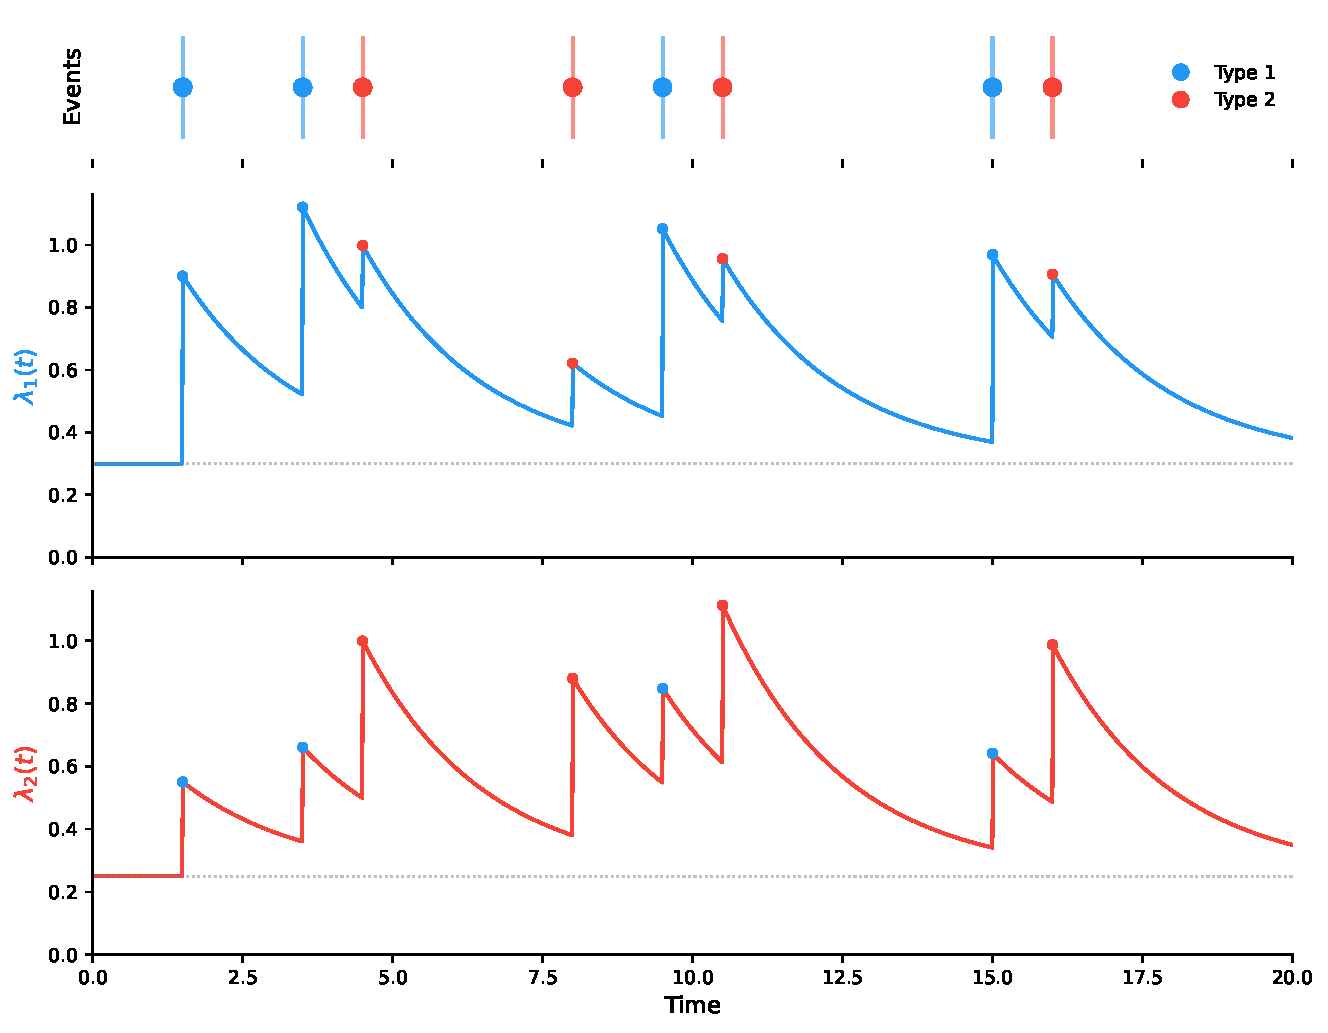
\includegraphics[width=0.9\linewidth]{figures/hawkes_illustration.pdf}
    \caption{Illustration of a multivariate Hawkes process with two event types. Each event causes a jump in the conditional intensity $\lambda(t)$, which decays exponentially. Events close in time accumulate their effects, and each type can excite events of both its own type and other types.}
    \label{fig:hawkesprocess}
\end{figure}

Neural models such as the Neural Hawkes Process \cite{mei2017neural}, using Long Short-Term Memory (LSTM) networks, emerged and began to capture complex relationships between events, outperforming linear models. Despite their broad applicability, these models face limitations common to recurrent networks, such as slow training and vanishing gradients.

Through resources such as telemetry or behavioral data collection from social networks, we now have an abundance of data, and training on long sequences is expensive and time-consuming, even with modern parallelizable techniques such as Transformers \cite{vaswani2017attention}. In language models, however, it is common to apply a technique called train short, test long \cite{press2022train}, which consists of training the model on short word sequences but testing on long sequences, always seeking to maintain model quality as measured by metrics such as perplexity. There is still no consolidated model in Temporal Point Processes (TPPs) that effectively addresses this problem.

The Transformer Hawkes Process (THP) \cite{zuo2020transformer} is a widely used Hawkes process model that, like the classical Transformer, uses embeddings with absolute times and is therefore not time-invariant, producing different results when executed at different times even with the same datasets and seeds. The Rotary Position Embedding-based Transformer Hawkes Process (RoTHP) \cite{dai2026rothp} addresses this problem through trigonometric rotation matrices \cite{su2024roformer}, which make it time-invariant but without the recency bias characteristic of a Hawkes process.

Returning to the language modeling domain, HoPE: Hyperbolic Rotary Positional Encoding for Stable Long-Range Dependency Modeling in Large Language Models \cite{dai2025hope} showed that hyperbolic functions combined with a learnable parameter to ensure exponential bias provide the model with stable perplexity even on sequences longer than those seen during training. The Hyperbolic Transformer Hawkes Process (HoTHP), our proposed model, pioneers this concept in the Hawkes process domain and shows that the inductive bias aligns with the very concept of the Hawkes process, demonstrating great stability on sequences longer than those seen during training, as measured by the log-likelihood.

\section{Background}

In this section, we present the fundamental concepts needed to understand the contribution of this work. We begin by defining temporal point processes and the Hawkes process, then discuss the cost function used to train these models, and trace the evolution of Hawkes models within machine learning, from parametric approaches to the Transformer-based architectures that motivate our work.

\subsection{Temporal Point Processes and the Hawkes Process}

A Temporal Point Process (TPP) is a stochastic model that describes sequences of events occurring in continuous time. Formally, a realization of a TPP is an ordered sequence of timestamps. When each event carries additional type information, we have a multivariate TPP, in which the sequence is given by $\mathcal{S} = \{(t_i, k_i)\}_{i=1}^N$, where $k_i$ represents the type of event $i$, $t$ the timestamp, and $N$ the number of events.

The central tool for describing the dynamics of a TPP is the conditional intensity function $\lambda(t \mid \mathcal{H}_t)$, which represents the instantaneous rate of event occurrence at time $t$, given the past events, that is, the probability of observing an event in the infinitesimal interval $[t, t + dt)$, where $\mathcal{H}$ represents all past events until $t$.

The Hawkes process \cite{hawkes1971spectra} is a particular case of TPP in which past events excite the occurrence of new ones. This phenomenon is called self-excitation. Its conditional intensity is defined by
%
\begin{equation}
\lambda(t) = \mu + \sum \varphi(t - t'),
\end{equation}
%
where $\mu > 0$ is the base intensity and $\varphi(\cdot)$ is the triggering kernel that quantifies the effect of each past event on the present intensity. The most common choice for $\varphi$ is the exponential kernel \cite{laub_hawkes_2025}:
%
\begin{equation}
\varphi(t) = \alpha \cdot \exp(-\beta \cdot t),
\end{equation}
%
with $\alpha$ controlling the magnitude of the effect and $\beta$ controlling the decay rate. It is important to note that the influence of a past event on the present intensity decays exponentially with elapsed time, and that events can inhibit, rather than excite, future occurrences. This property will be central to the motivation of HoTHP.

\subsection{Log-Likelihood in Point Processes}

The standard cost function for training TPP models is the log-likelihood. Given a sequence of events $\{t_1, \ldots, t_N\}$ observed in an interval $[0, T]$, the log-likelihood is defined as:
%
\begin{equation}
\mathcal{L} = \sum_{i=1}^{N} \log \lambda(t_i) - \int_0^T \lambda(t) \, dt.
\end{equation}
%
The first term rewards the model for assigning high intensity at the instants where events actually occurred. The second term penalizes the model for maintaining high intensity in regions where there are no events. For convenience, we minimize the negative log-likelihood (NLL), which is the metric we use in the experiments.

\subsection{From Simple Parametric Models to Transformers}

The first models for Hawkes processes were parametric and assumed a specific form for the kernel, with the exponential being the most commonly used. Although mathematically tractable, these approaches have limited expressiveness and do not capture well complex dependencies between events of different types \cite{shchur2021neural}.

To overcome this limitation, neural approaches emerged. The Neural Hawkes Process (NHP) \cite{mei2017neural} uses a Recurrent Neural Network (RNN) LSTM to model the conditional intensity, allowing it to capture complex and long-range dependencies. However, the sequential nature of LSTMs makes  parallelization more difficult and training slow on long sequences.

The Transformer Hawkes Process (THP) \cite{zuo2020transformer} brought the self-attention mechanism of Transformers to the TPP context, enabling parallel processing and capture of dependencies between distant events. To represent the temporal position of each event, the THP uses a sinusoidal encoding applied directly to the absolute time of each event:
%
\begin{equation}
[\bm{z}(t_j)]_i =
\begin{cases}
\cos\!\left(\frac{t_j}{10000^{(i-1)/d}}\right), & \text{if } i \text{ is odd,} \\[4pt]
\sin\!\left(\frac{t_j}{10000^{i/d}}\right), & \text{if } i \text{ is even,}
\end{cases}
\end{equation}
%
where $d$ is the model dimension. The problem with this approach is that it operates on absolute timestamps. Shifting all timestamps by a constant $\sigma$ changes the computations and, consequently, the attention scores and the model predictions.

\subsection{RoTHP: Time Invariance via Rotation}

RoTHP \cite{dai2026rothp} solves the time-invariance problem by adapting RoPE \cite{su2024roformer} to continuous timestamps. Instead of adding a positional encoding to the event time, RoTHP rotates the query $\bm{q}$ and key $\bm{k}$ vectors using a rotation matrix $\bm{R}$:
%
\begin{equation}
\bm{R}(t_i) =
\begin{pmatrix}
\cos t_i\theta_1 & \sin t_i\theta_1 & \cdots & 0 & 0 \\
-\sin t_i\theta_1 & \cos t_i\theta_1 & \cdots & 0 & 0 \\
\vdots & \vdots & \ddots & \vdots & \vdots \\
0 & 0 & \cdots & \cos t_i\theta_{d/2} & \sin t_i\theta_{d/2} \\
0 & 0 & \cdots & -\sin t_i\theta_{d/2} & \cos t_i\theta_{d/2}
\end{pmatrix},
\end{equation}
%
where the $\theta_l$ are learnable frequencies. Since the attention is computed by the inner product of $Q$ and $K$, we have:
%
\begin{equation}
\bm{q}_i^\top \bm{R}(t_i)^\top \bm{R}(t_j) \, \bm{k}_j = \bm{q}_i^\top \bm{R}(t_j - t_i) \, \bm{k}_j.
\end{equation}
%
This ensures that the attention score depends only on the temporal difference $\Delta t = t_j - t_i$, respecting time invariance.

However, the cosine and sine functions are oscillatory. As $\Delta t$ grows, the attention score oscillates periodically, as shown in Fig-\ref{fig:kernel_alignment}. This means that two temporally close events may receive a lower attention score than distant events, depending on the phase of the oscillation. This behavior contradicts the natural exponential decay of the Hawkes process, in which the influence of past events should decrease monotonically with time.

\begin{figure}[t]
\centering
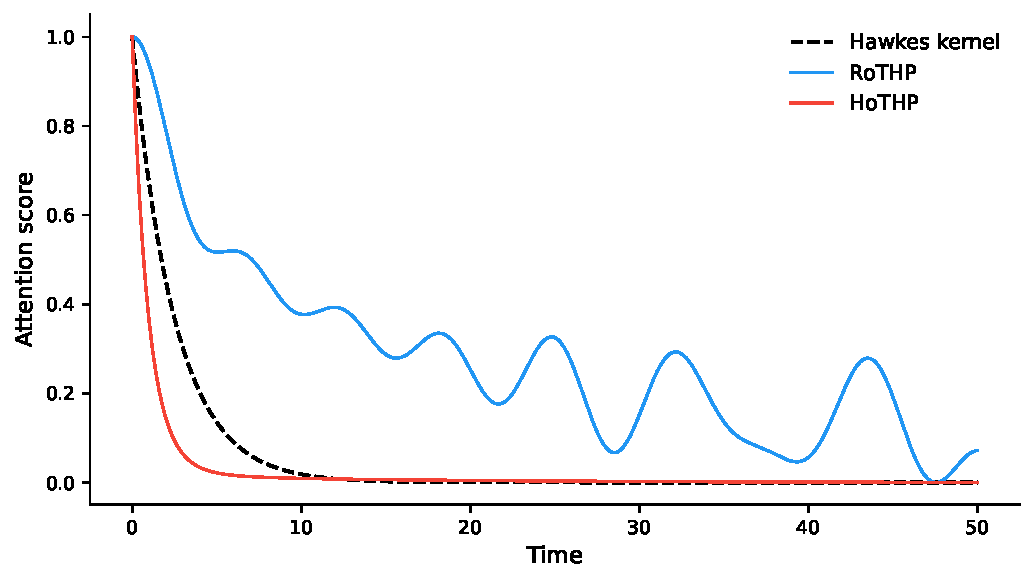
\includegraphics[width=0.72\textwidth]{figures/kernel_alignment.pdf}
\caption{Normalized attention profile of each model compared to the true exponential kernel $e^{-\beta \Delta t}$. HoTHP aligns better with the real kernel than RoTHP.}
\label{fig:kernel_alignment}
\end{figure}

This problem worsens in the length extrapolation scenario. When the model is tested on sequences longer than those seen during training, the temporal differences can reach values that were never observed during training. Since the trigonometric function oscillates in these regions, the model has no guarantee of generalizing correctly, and in practice performance degrades.

\subsection{Length Extrapolation}

Before presenting HoTHP, it is necessary to clarify the problem it aims to solve. In this section, we define length extrapolation in the context of TPPs, argue how a recency bias applied to the attention mechanism is suitable for Hawkes processes, and empirically demonstrate that rotational models based on trigonometric rotation, despite being time-shift invariant, do not possess this characteristic.

We adapt the definition from Attention with Linear Biases (ALiBi) \cite{press2022train} to the TPP scenario. Let $L$ be the length (in number of events) of the sequences used during training and $L_{test}$ the length of the sequences used for testing. We say that a model extrapolates efficiently when its performance remains stable as the ratio $L_{test}/L$ grows, in the case of TPPs, considering the log-likelihood as the cost function. Given the quadratic nature of the Transformer architecture, training the model on very long sequences can become infeasible.

As we have seen, RoTHP solves the time-invariance issue, but the oscillatory nature of its trigonometric functions prevents a monotonic decay in the attention scores. This motivates the search for a positional encoding that combines time invariance with an exponential decay bias, aligned with the structure of the Hawkes process itself.


\section{Hyperbolic Rotary Position Embedding-based Transformer Hawkes Process for Length Extrapolation (HoTHP)}

HoTHP is built upon three basic principles: the attention score must depend only on the temporal difference between events, ensuring invariance to time shifts; the score must decrease monotonically, following the bias introduced by the original Hawkes process; and the decay must be part of the model structure and not merely an additional layer. We adopt the hyperbolic kernel from HoPE \cite{dai2025hope} and adapt it for TPPs by reformulating the product $q^T\boldsymbol{B}(\theta,m-n)k$ directly as a function of the temporal delta, unlike RoTHP, which pre-rotates $\bm{q}$ and $\bm{k}$ before sending them to the attention mechanism.

\subsection{From Trigonometric Rotation to Hyperbolic Rotation}

As seen in Section 2.4, the rotation matrix $\bm{R}(t_i)$ of RoTHP \cite{dai2026rothp,dai2025hope} is block-diagonal, composed of $2 \times 2$ trigonometric rotation blocks. For each pair of dimensions $(2j{-}1, 2j)$, the corresponding block applied to a temporal difference $\Delta t$ is:

%
\begin{equation}
\bm{R}_j(\Delta t) = \begin{bmatrix} \cos(\theta_j \Delta t) & \sin(\theta_j \Delta t) \\ -\sin(\theta_j \Delta t) & \cos(\theta_j \Delta t) \end{bmatrix}.
\end{equation}
%
This block ensures time invariance, since the attention score depends only on $\Delta t = t_i - t_j$.

HoPE \cite{dai2025hope} proposes replacing the trigonometric rotation with a hyperbolic rotation. The $2 \times 2$ block becomes:
%
\begin{equation}
\bm{B}_j(\Delta t) = \begin{bmatrix} \cosh(\theta_j \Delta t) & \sinh(\theta_j \Delta t) \\ \sinh(\theta_j \Delta t) & \cosh(\theta_j \Delta t) \end{bmatrix}.
\label{eq:boost}
\end{equation}
%

The fundamental difference is that $\cosh$ and $\sinh$ are monotonic functions (for $\Delta t > 0$), unlike $\cos$ and $\sin$, which oscillate. This eliminates the undesirable oscillations in the attention score. However, we cannot use the block $\bm{B}_j$ directly because, unlike the trigonometric rotation, the hyperbolic rotation is not an orthogonal transformation; moreover, the inner product of $\bm{q}$ and $\bm{k}$ grows with $|\Delta t|$ instead of decaying \cite{dai2025hope}. This means that distant events would receive higher scores than nearby events, which is the opposite of the desired behavior.

To solve this problem, HoPE \cite{dai2025hope} introduces a learnable parameter $\theta'$ and applies damping factors to the $\bm{q}$ and $\bm{k}$ vectors, with $\bm{q}$ at position $m$ multiplied by $e^{-m\theta'}$, and $\bm{k}$ by $e^{+m\theta'}$. When we compute the attention score between positions $m$ and $n$, these factors combine:
%
\begin{equation}
g(\bm{x}_m, \bm{x}_n, n{-}m) = e^{-(m-n)\theta'} \; \bm{q}^\top \bm{B}(\theta, m{-}n) \; \bm{k}.
\label{eq:hope_score}
\end{equation}
%
Adapting for TPPs, we replace the discrete positions $m, n$ with the continuous timestamps $t_i, t_j$, and the difference $m - n$ with the temporal delta $\Delta t = t_i - t_j$. The attention score becomes:
%
\begin{equation}
g(\Delta t) = e^{-\Delta t \cdot \theta'} \; \bm{q}^\top \, \bm{B}(\theta ,\Delta t) \; \bm{k}.
\label{eq:kernel_completo}
\end{equation}
%
For the damping to dominate the growth of $\cosh$, it is required that $\theta' > \max \theta$. Under this condition, the score decays monotonically with $\Delta t$, like the exponential kernel of the Hawkes process, where recent events are naturally more influential than distant events.


\subsection{HoTHP Attention Score}

Substituting the definition of $\bm{B}_j$ (Eq.~\ref{eq:boost}) into Eq.~\ref{eq:kernel_completo}, the attention score for dimension pair $j$ becomes:

%
\begin{equation}                                                        g_j(\Delta t) = e^{-|\Delta t|\theta'}
\!\left[
\underbrace{(q_1 k_1 + q_2 k_2)}_{\text{cosh part}} \cosh(\theta_j \Delta t)
+ \underbrace{(q_1 k_2 + q_2 k_1)}_{\text{sinh part}} \sinh(\theta_j \Delta t)                                                                      
\right].                                                                    \label{eq:score_par}
\end{equation}
%      

As in HoPE, we keep the parameter $\theta'$, enforcing the constraint $\theta' > \max \theta$ throughout training. Since $\theta'$ is a learnable parameter, we cannot simply fix its value. To enforce this constraint automatically during training, we parameterize $\theta'$ as:
%
\begin{equation}
\theta' = \mathrm{softplus}(\theta'_{\mathrm{raw}}) + \max(\theta) + \epsilon,
\label{eq:theta_prime}
\end{equation}
%
where $\theta'_{\mathrm{raw}}$ is the learnable parameter and $\epsilon = 10^{-4}$ is a safety margin. In this way, we structurally guarantee that $\theta'$ is greater than any value of $\theta$ and, therefore, guarantee the exponential decay.

\subsection{Temporal Normalization}

Different datasets have very distinct time scales: in social networks, the intervals between events can be on the order of milliseconds, while in seismic data they can be on the order of days. If we used raw timestamps in the hyperbolic kernel, the values of $\theta \Delta t$ would be on incompatible scales and the model would not work well without manual tuning.

To address this, we normalize the timestamps before computing the attention scores. First, we shift the timestamps so that the sequence starts at zero. Then, we divide each timestamp by the mean inter-event interval observed up to that point.

After this normalization, the mean inter-event interval is close to $1{.}0$, regardless of the original scale of the data.

\subsection{Full Architecture}

The HoTHP architecture follows the encoder structure of the Transformer \cite{vaswani2017attention}, adapted for temporal point processes. Each event $(t_i, k_i)$ is represented by a learned embedding of type $k_i$. Unlike THP \cite{zuo2020transformer}, timestamps are not added to the embedding; temporal information is incorporated exclusively through the hyperbolic kernel in the attention mechanism.

The model uses $N$ stacked encoder layers, each composed of a multi-head attention block followed by a feed-forward network. The attention block computes scores via the hyperbolic kernel, using the normalized temporal differences. A causal mask is applied to ensure that each event attends only to previous events. The conditional intensity for each event type $k$ is computed as:
%
\begin{equation}
\lambda_k(t \mid \mathcal{H}_t) = f_k\!\left(\underbrace{\alpha_k \frac{(t - t_j)}{t_j}}_{\text{current}} + \underbrace{\bm{w}_k^\top \bm{h}(t_j)}_{\text{history}} + \underbrace{b_k}_{\text{base}}\right),
\label{eq:intensidade}
\end{equation}
%
where $\bm{h}(t_j)$ is the encoder output representation for event $j$, $\alpha_k$, $\bm{w}_k$, and $b_k$ are learnable parameters, and $f_k = \mathrm{softplus}$ is the activation function that ensures positivity of the intensity, following the THP formulation \cite{zuo2020transformer}.

The main difference between HoTHP and RoTHP lies in how temporal information enters the attention mechanism. RoTHP individually pre-rotates the $\bm{q}$ and $\bm{k}$ vectors using the trigonometric matrices $\bm{R}(t_i)$ and $\bm{R}(t_j)$, and then computes the standard dot product, so that the dependence on $\Delta t$ is mathematically guaranteed. In HoTHP, the attention score $\bm{q}^\top \bm{B}(\Delta t) \bm{k}$ is formulated directly as a function of the temporal difference between each pair of events, which allows incorporating the decay factor $e^{-\Delta t \, \theta'}$ into the kernel structure itself.

\section{Experiments}

\subsection{Experimental Setup}

We generate event sequences from multivariate Hawkes processes with $K=2$ event types and exponential kernel. To evaluate the model behavior under different regimes of temporal dependence, we define two scenarios. In the slow decay scenario, the influence of past events persists for a long time, so that distant events still contribute significantly to the present intensity. In the fast decay scenario, only recent events exert relevant influence. For each scenario, we generate 500 training sequences, 150 validation sequences, and 200 test sequences.

Training follows the \textit{train short, test long} technique, inspired by \cite{press2022train}. To systematically evaluate the extrapolation capability, we sweep over multiple training lengths ($L \in \{10, 20, 50, 100\}$) and extrapolation factors ($2\times$, $5\times$, $10\times$), resulting in test sequences ranging from 20 to 1{,}000 events. The NLL is computed over the full sequence, allowing a direct measurement of the model's length extrapolation capability across different combinations of training length and extrapolation ratio.

We compare HoTHP with RoTHP \cite{dai2026rothp}, both implemented on the EasyTPP framework \cite{xue2024easytpp}. The only difference between the models is the positional kernel used in the attention mechanism. All experiments are repeated with $N=5$ distinct seeds and we report mean $\pm$ standard deviation. Statistical significance is assessed via the Wilcoxon signed-rank test (one-sided), a non-parametric paired test appropriate for small sample sizes.

\subsection{Slow Decay vs.\ Fast Decay}

Table~\ref{tab:main_results} presents the NLL results for both models in the two decay scenarios, evaluated on sequences of different lengths. Fig.~\ref{fig:main_result} illustrates the evolution of the NLL as the test length grows.

\begin{table}[t]
\centering
\caption{NLL (mean $\pm$ standard deviation, $N=5$ seeds) for the slow and fast decay scenarios. Values in \textbf{bold} indicate the best result in each column per process group. Lower values are better. Statistical significance assessed via Wilcoxon signed-rank test ($^{*}$\,$p<0.05$).}
\label{tab:main_results}
\begin{tabular}{llcccc}
\toprule
Process & Model & $1\times$ & $2\times$ & $5\times$ & $10\times$ \\
\midrule
\multirow{2}{*}{Slow} & RoTHP & \textbf{1.685 $\pm$ 0.004} & 1.719 $\pm$ 0.009 & 1.757 $\pm$ 0.024 & 1.779 $\pm$ 0.035 \\
 & HoTHP & 1.693 $\pm$ 0.009 & \textbf{1.698 $\pm$ 0.021} & \textbf{1.713 $\pm$ 0.032} & \textbf{1.724 $\pm$ 0.038} \\
\midrule
\multirow{2}{*}{Fast} & RoTHP & \textbf{1.677 $\pm$ 0.003} & 1.994 $\pm$ 0.126 & 2.111 $\pm$ 0.186 & 2.246 $\pm$ 0.246 \\
 & HoTHP & 1.692 $\pm$ 0.006 & \textbf{1.693 $\pm$ 0.009}$^{*}$ & \textbf{1.694 $\pm$ 0.010}$^{*}$ & \textbf{1.695 $\pm$ 0.011}$^{*}$ \\
\bottomrule
\end{tabular}
\end{table}

\begin{figure}[t]
\centering
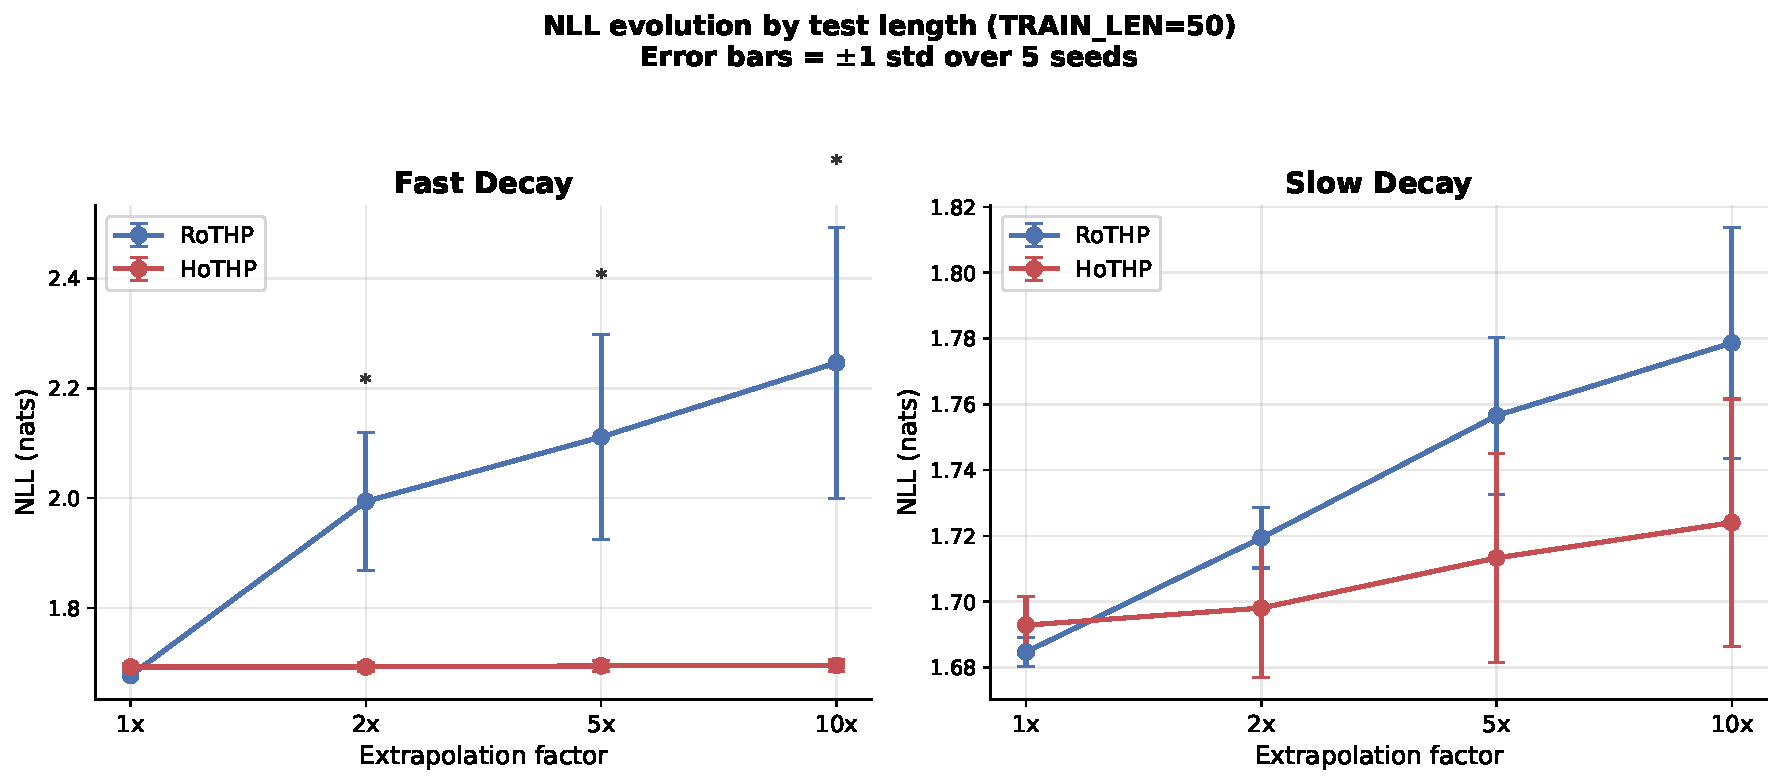
\includegraphics[trim={0 0 0 2.5cm},clip,width=0.8\textwidth]{figures/main_result.pdf}
\caption{NLL evolution as a function of test length for the slow decay (left) and fast decay (right) scenarios. Error bars indicate $\pm 1$ standard deviation over 5 seeds.}
\label{fig:main_result}
\end{figure}

In the fast decay scenario, HoTHP consistently outperforms RoTHP across all extrapolation scales, with statistically significant differences (Wilcoxon $p=0.031$) at $2\times$, $5\times$, and $10\times$. At the $10\times$ scale, the NLL difference is $0.551$ nats. The HoTHP NLL remains essentially flat across all scales ($\approx 1.69$), while RoTHP degrades from $1.68$ at $1\times$ to $2.25$ at $10\times$. Beyond the difference in means, the standard deviations reveal an important difference in model stability. RoTHP exhibits a standard deviation of $0.246$ at the $10\times$ scale, compared to only $0.011$ for HoTHP. This suggests that the trigonometric kernel of RoTHP is sensitive to extrapolation beyond horizons seen during training, while the hyperbolic kernel of HoTHP maintains consistent behavior regardless of the seed.

In the slow decay scenario, HoTHP also achieves lower NLL than RoTHP at all extrapolation scales, although the differences are smaller and do not reach statistical significance for $L=50$ ($p=0.062$ at $10\times$). This suggests that the exponential decay bias of HoTHP provides a benefit even when the generating process has slow decay, though the effect is less pronounced because the oscillatory behavior of the trigonometric kernel is less harmful when temporal differences are smaller.

These results indicate that the decay bias of HoTHP aligns with the structure of the Hawkes process with exponential kernel, enabling more stable extrapolation in both decay regimes, with a particularly large advantage in processes with fast decay.

\subsection{Complementary Analyses}

Fig.~\ref{fig:kernel_alignment} compares the attention profile of each model with the true exponential kernel of the generating process. RoTHP exhibits an oscillatory profile, while HoTHP exhibits a decreasing profile closer to the real kernel. This shows that the hyperbolic kernel is able to learn an attention profile more aligned with the exponential decay of the Hawkes process.

Fig.~\ref{fig:grid_heatmap} summarizes the HoTHP advantage (NLL\textsubscript{RoTHP} $-$ NLL\textsubscript{HoTHP}) across all combinations of training length and extrapolation factor. In the fast decay scenario, HoTHP is significantly better in all 12 combinations (Wilcoxon $p=0.031$), with the advantage growing as the training length decreases and the extrapolation factor increases. In the slow decay scenario, 9 out of 12 combinations are significant at $p<0.05$, confirming that the benefit of the hyperbolic kernel is not restricted to fast decay processes.

\begin{figure}[!htb]
\centering
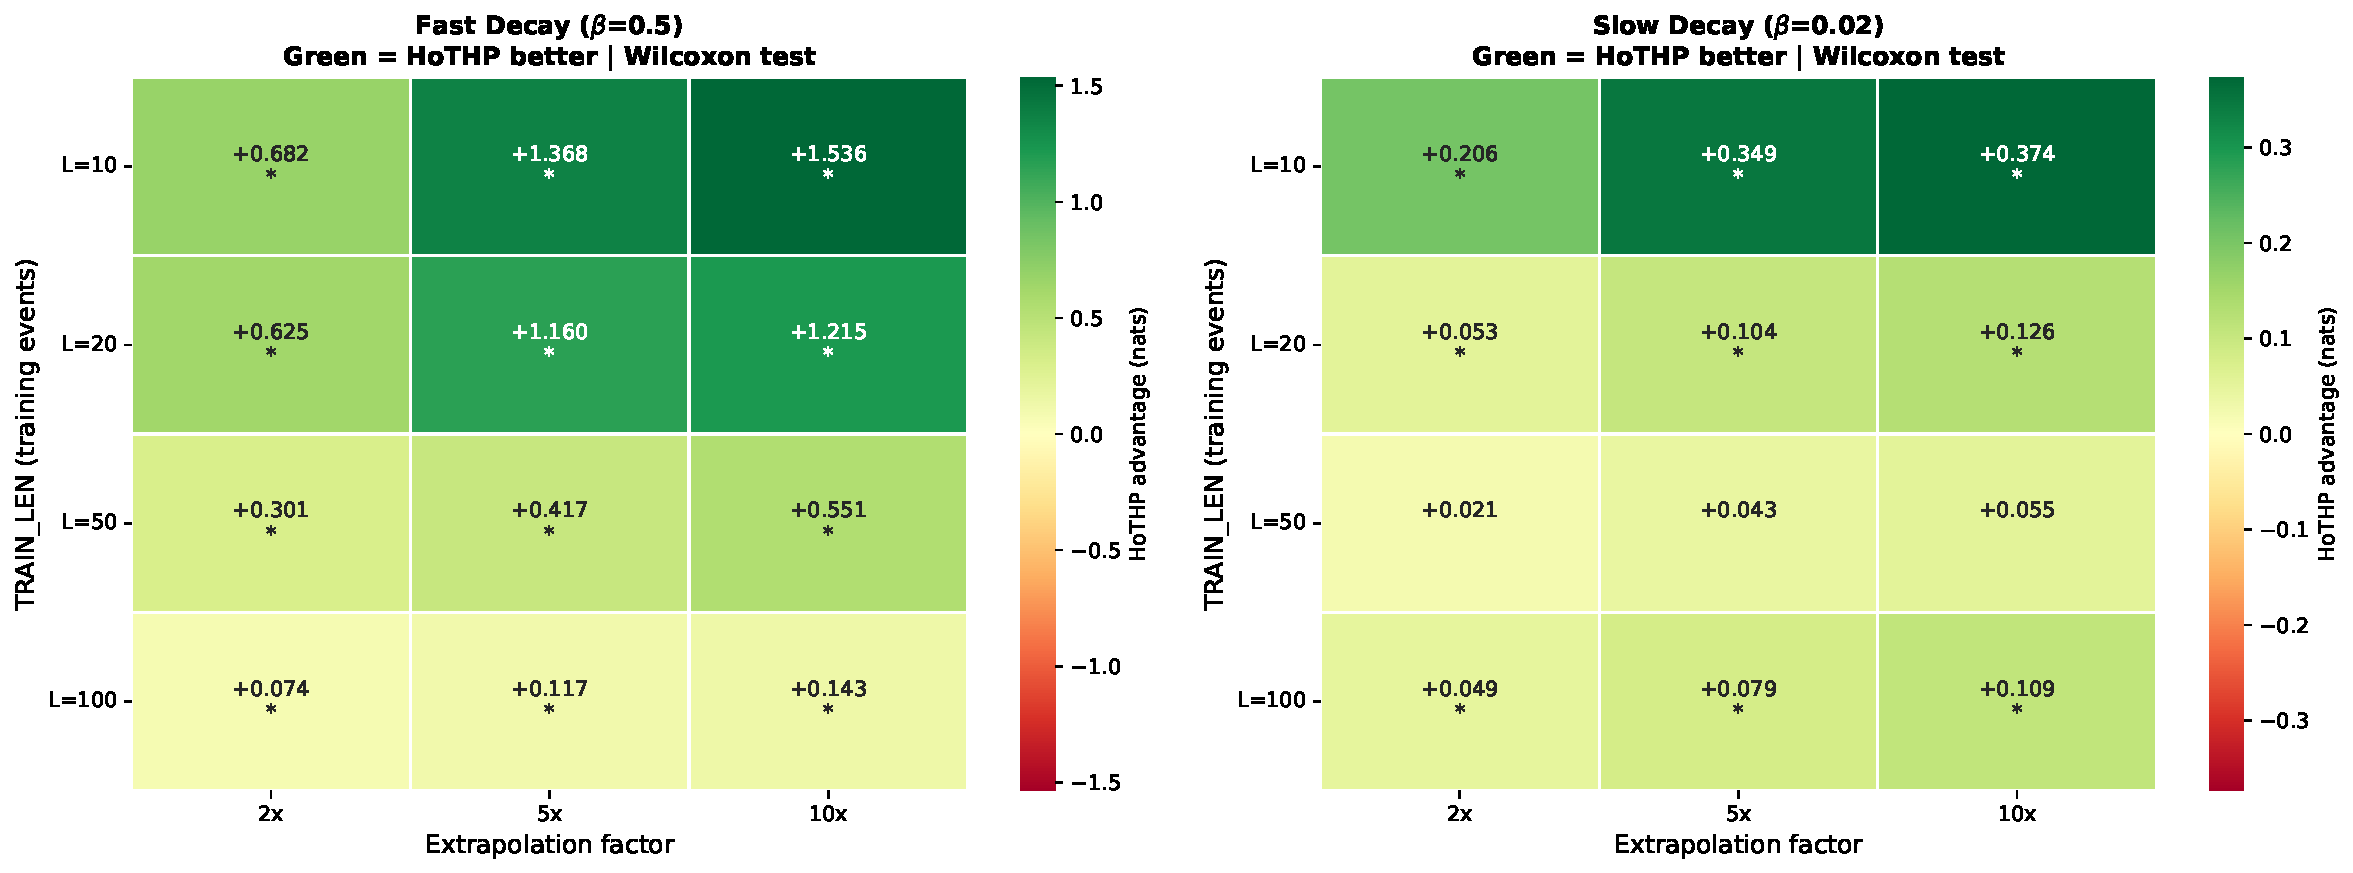
\includegraphics[trim={0 0 20cm 0},clip,width=0.8\textwidth]{figures/grid_heatmap_combined.pdf}
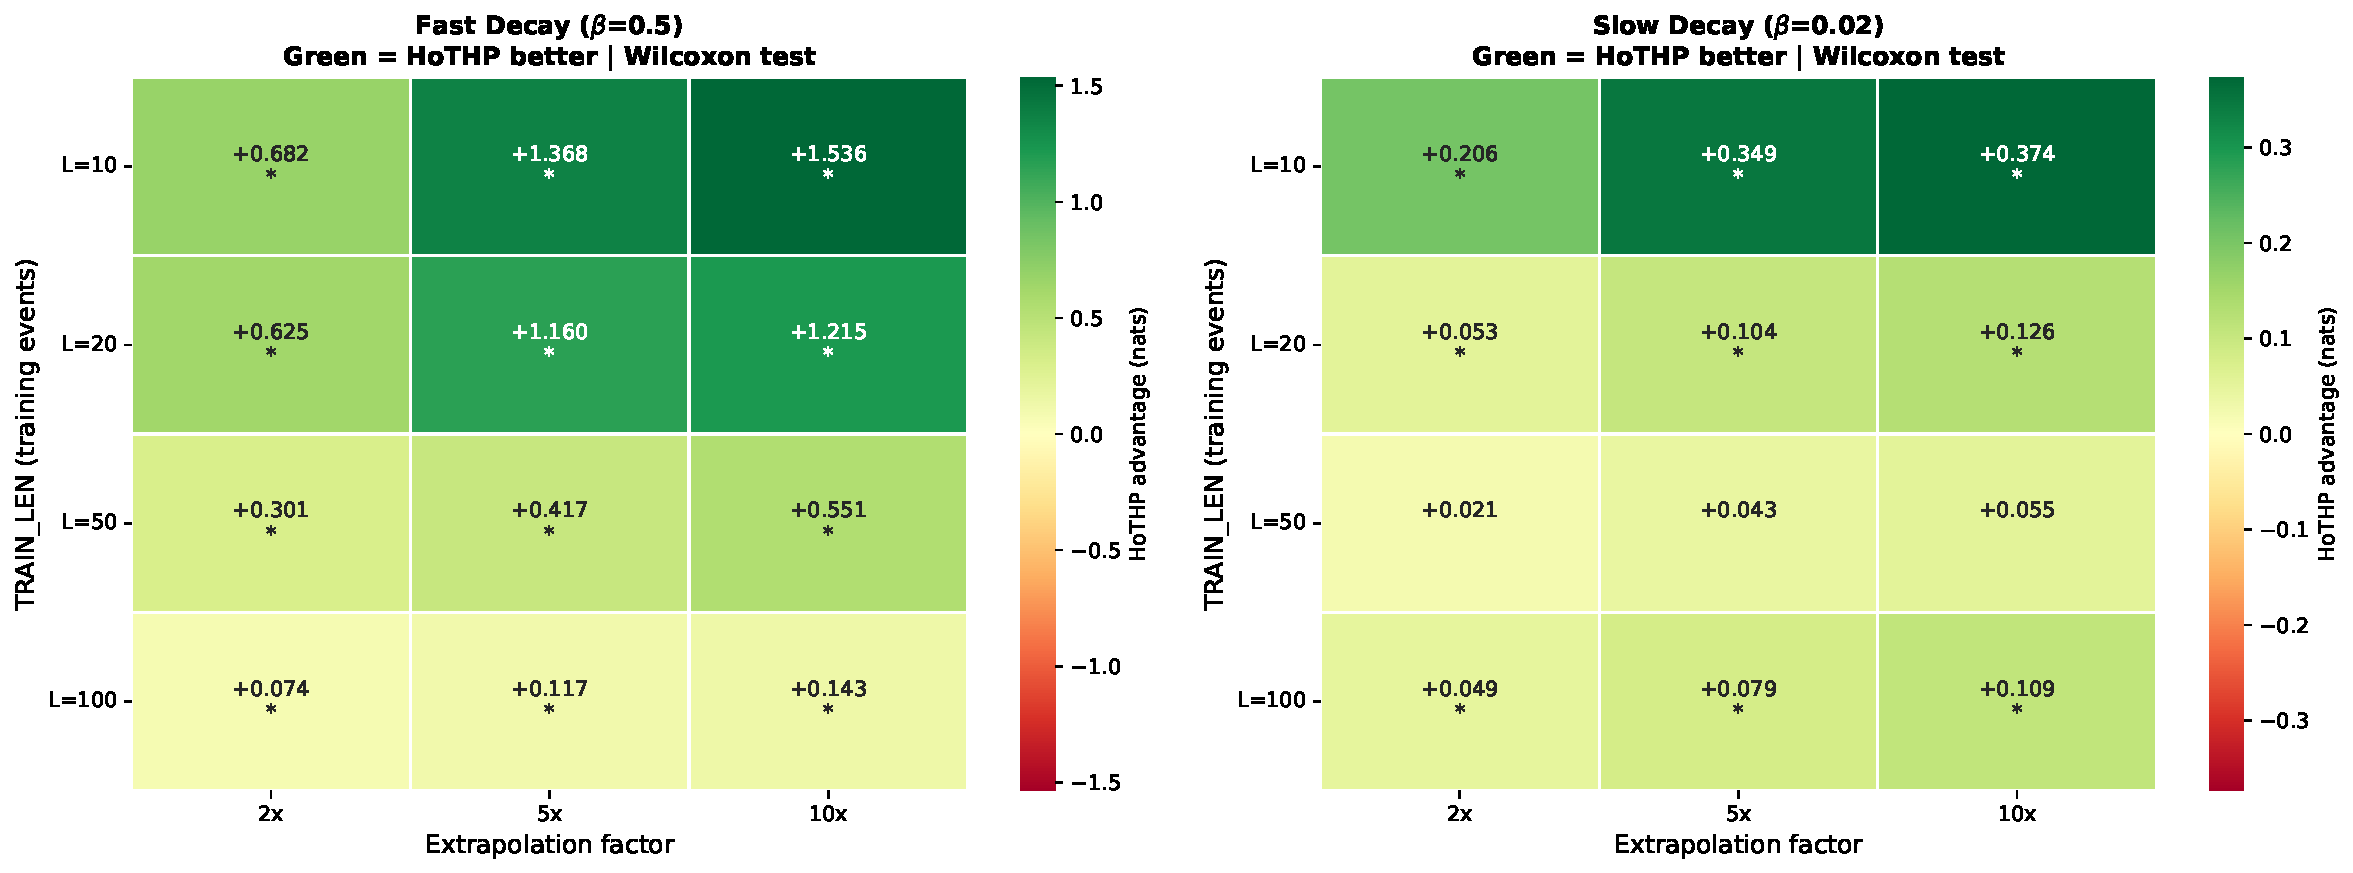
\includegraphics[trim={20cm 0 0 0},clip,width=0.8\textwidth]{figures/grid_heatmap_combined.pdf}
\caption{HoTHP advantage over RoTHP (NLL difference in nats) across training lengths and extrapolation factors. Green indicates HoTHP is better. Asterisks denote Wilcoxon signed-rank significance ($^{*}$\,$p<0.05$). Left: fast decay. Right: slow decay.}
\label{fig:grid_heatmap}
\end{figure}

\begin{figure}[!htb]
\centering
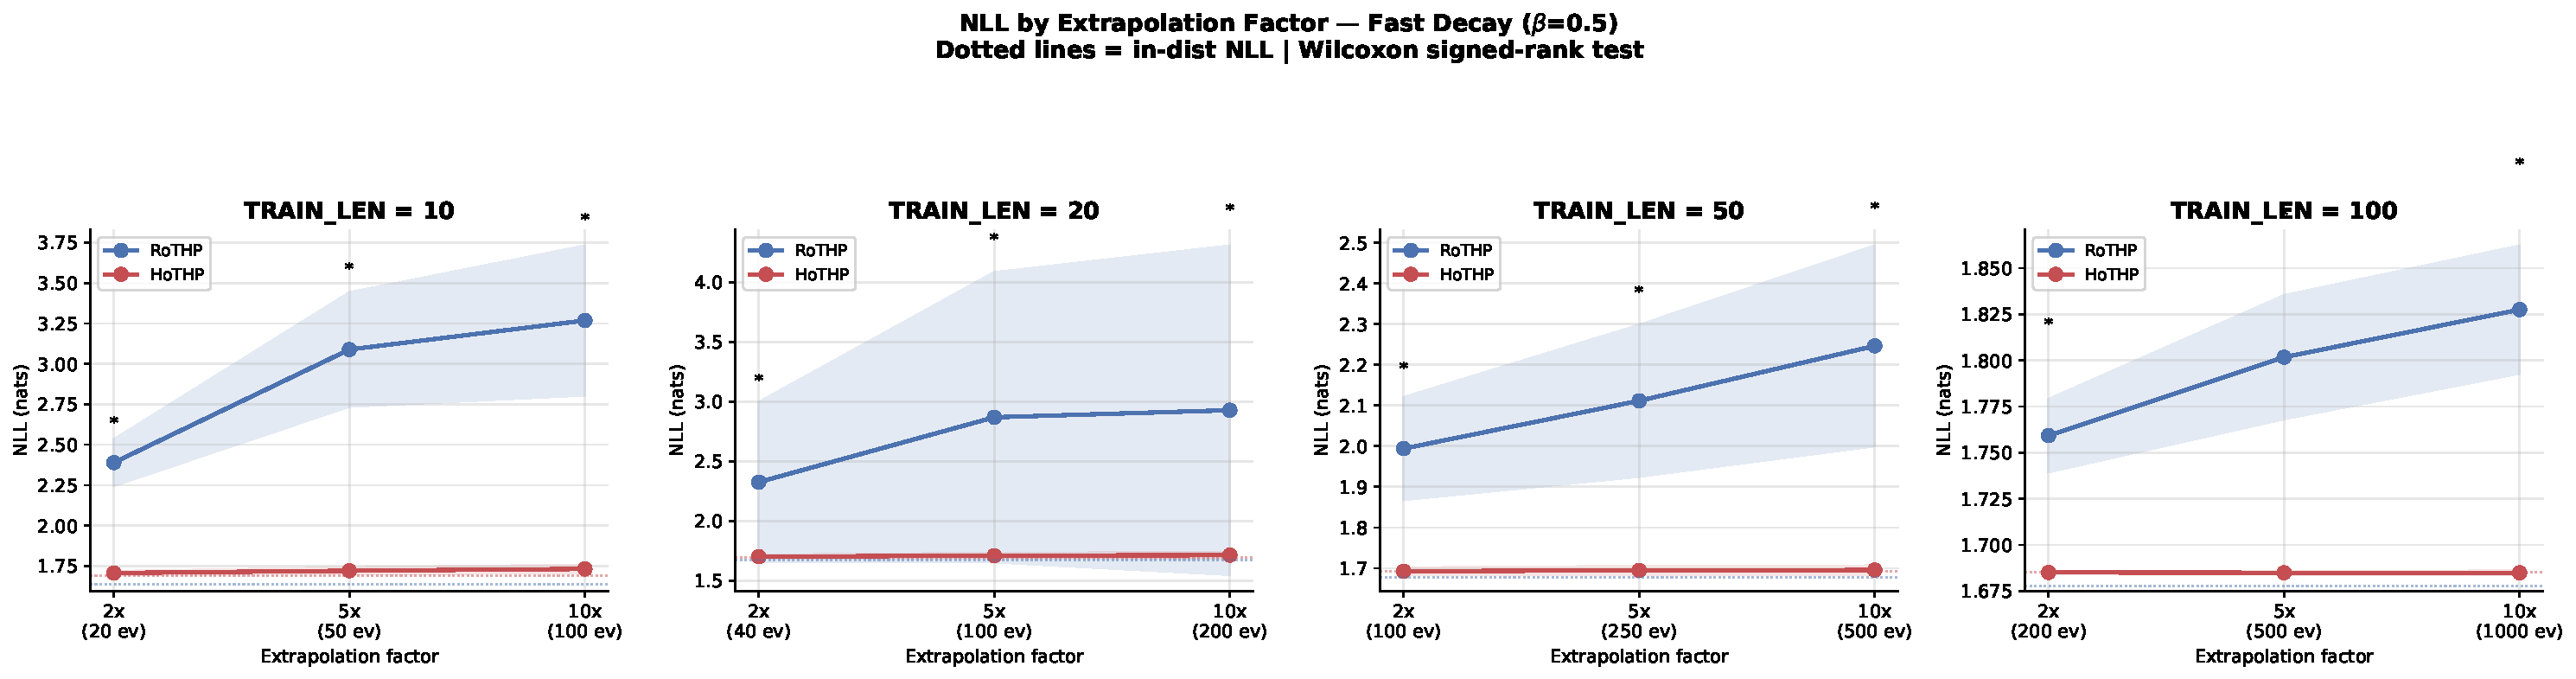
\includegraphics[trim={0 0 25cm 3cm},clip,width=0.9\textwidth]{figures/grid_nll_lines_fast.pdf}
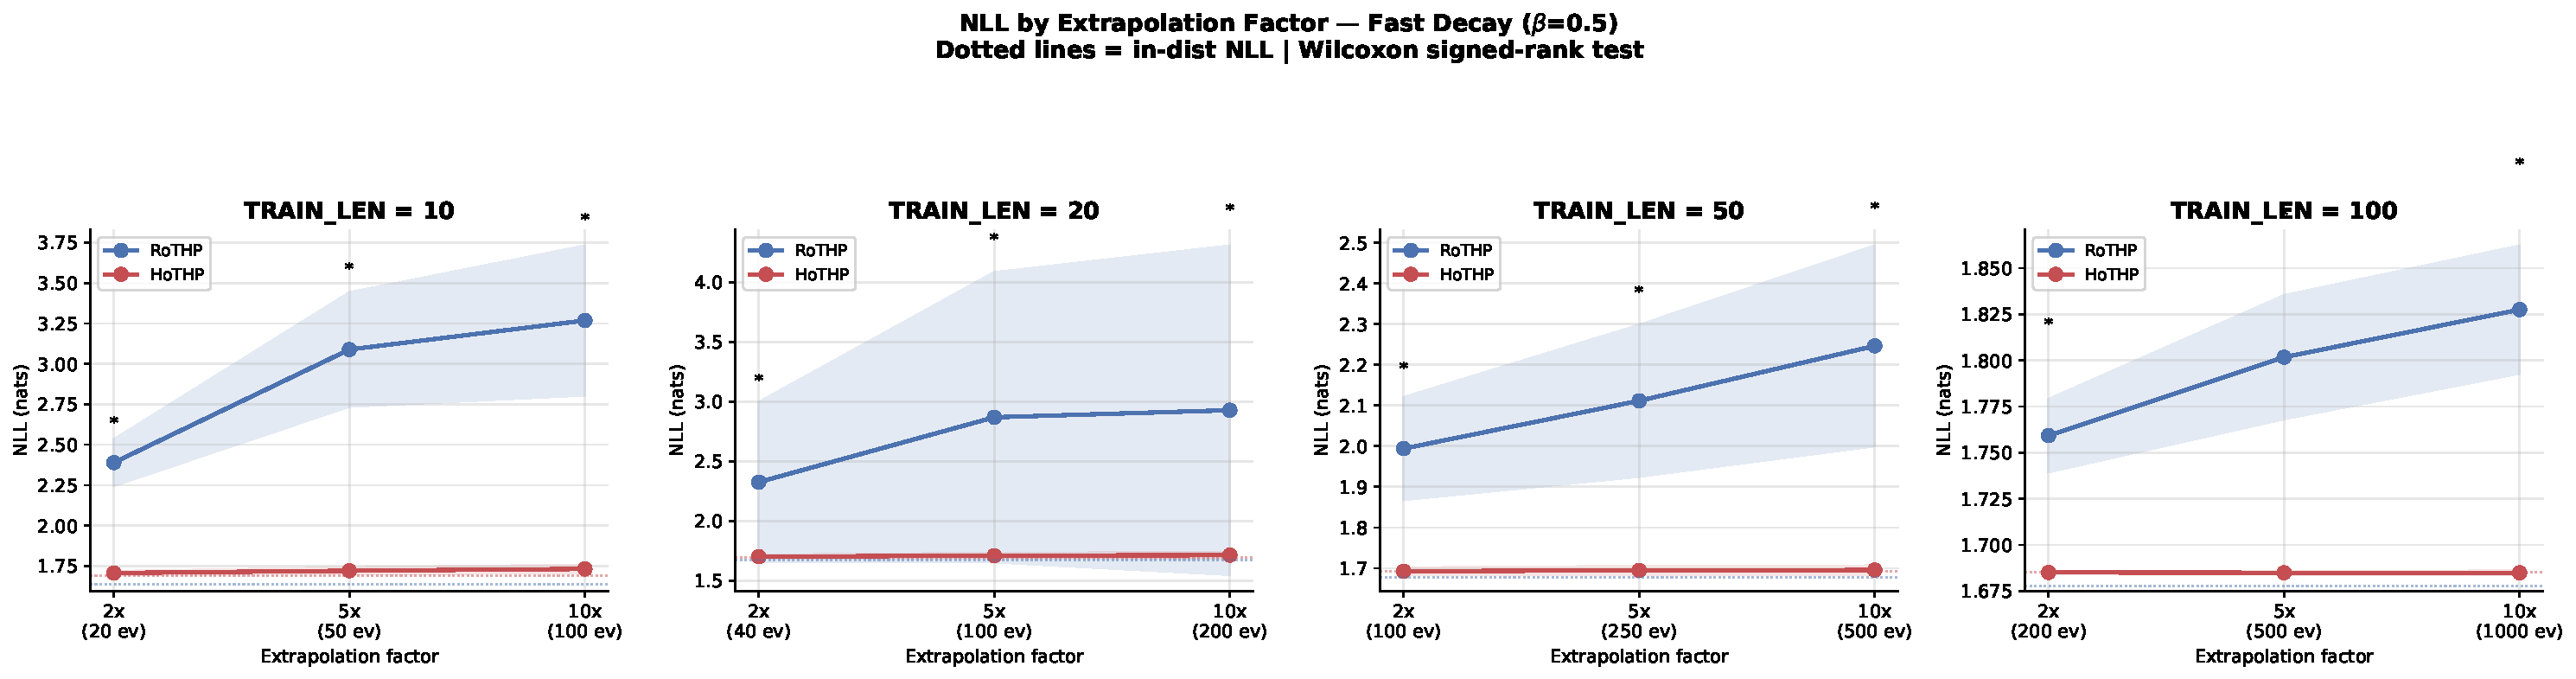
\includegraphics[trim={25cm 0 0 3cm},clip,width=0.9\textwidth]{figures/grid_nll_lines_fast.pdf}
\caption{NLL by extrapolation factor for each training length in the fast decay scenario. Shaded areas indicate $\pm 1$ standard deviation over 5 seeds. Dotted lines show in-distribution NLL. Asterisks denote Wilcoxon significance ($^{*}$\,$p<0.05$).}
\label{fig:grid_lines_fast}
\end{figure}

\begin{figure}[!htb]
\centering
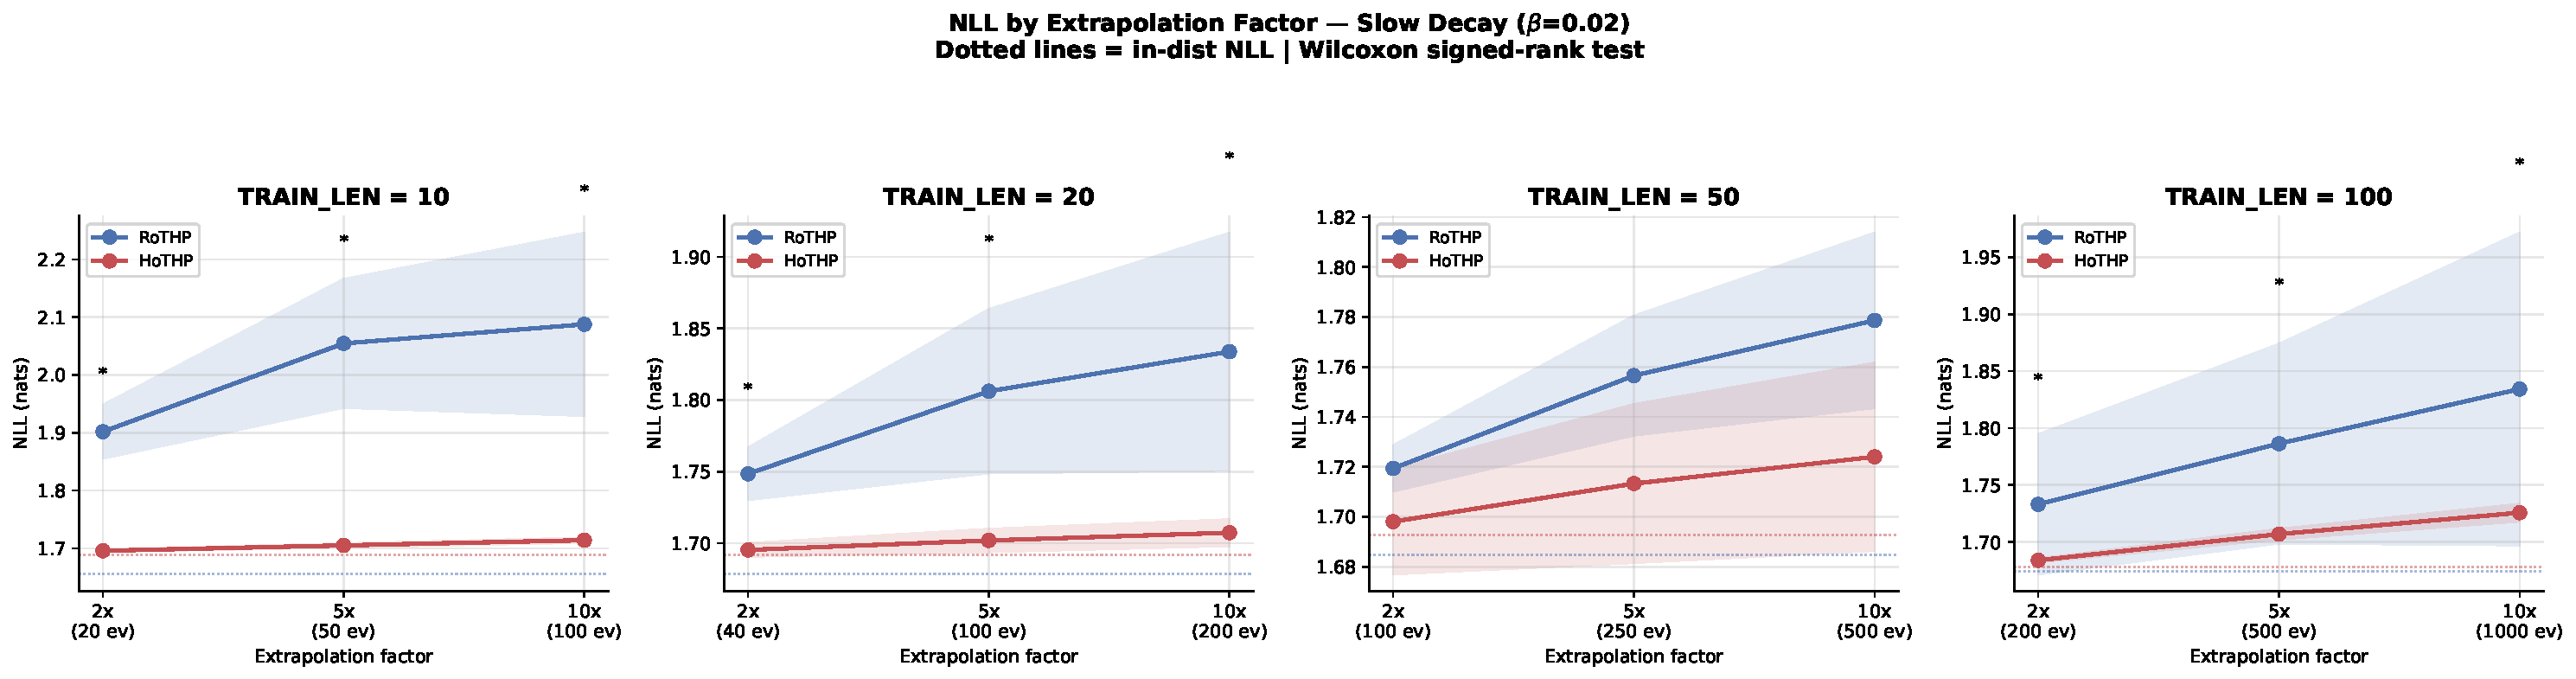
\includegraphics[trim={0 0 25cm 3cm},clip,width=0.9\textwidth]{figures/grid_nll_lines_slow.pdf}
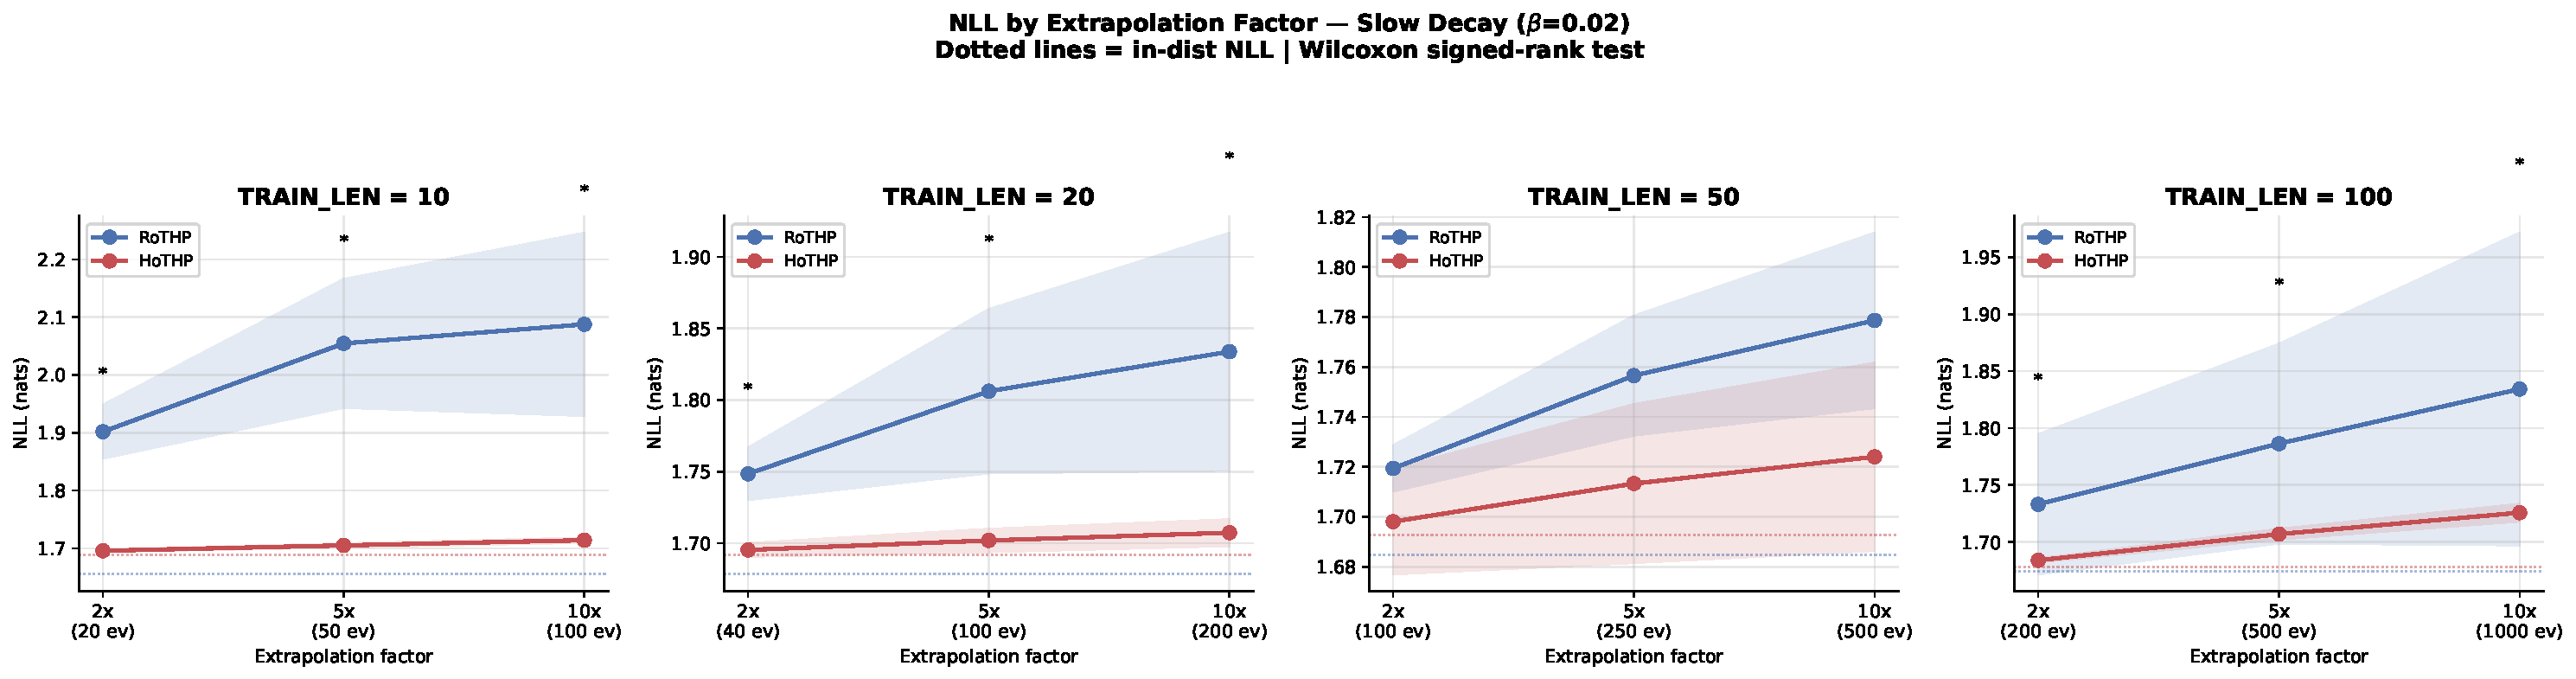
\includegraphics[trim={25cm 0 0 3cm},clip,width=0.9\textwidth]{figures/grid_nll_lines_slow.pdf}
\caption{NLL by extrapolation factor for each training length in the slow decay scenario. Shaded areas indicate $\pm 1$ standard deviation over 5 seeds. Dotted lines show in-distribution NLL. Asterisks denote Wilcoxon significance ($^{*}$\,$p<0.05$).}
\label{fig:grid_lines_slow}
\end{figure}

Figs.~\ref{fig:grid_lines_fast} and~\ref{fig:grid_lines_slow} show the NLL evolution for each training length individually. In the fast decay scenario (Fig.~\ref{fig:grid_lines_fast}), RoTHP degrades sharply across all training lengths, while HoTHP remains stable. The effect is most dramatic for shorter training sequences ($L=10$, $L=20$), where RoTHP reaches NLL values above $3.0$ at $10\times$ extrapolation. In the slow decay scenario (Fig.~\ref{fig:grid_lines_slow}), the gap between the two models is narrower but HoTHP consistently maintains lower NLL. The only case where the confidence bands overlap substantially is $L=50$, where the HoTHP advantage does not reach statistical significance.

%\FloatBarrier

\section{Related Work}

Our contribution in neural networks for TPPs involves concepts drawn from the most recent advances in positional encoding for Transformers. Although parallel, these lines of research have maintained a recurring dialogue on advances in positional encoding originally proposed within the context of language models and their adaptations to TPP scenarios, and these adaptations have represented important performance leaps in the area. THP \cite{zuo2020transformer} established this pattern by adapting the original Transformer architecture \cite{vaswani2017attention} to continuous event sequences. RoTHP \cite{dai2026rothp} continued this trend by adapting RoPE \cite{su2024roformer} to continuous timestamps, addressing the fragility of THP with temporal shifts. 

ALiBi \cite{press2022train} introduced a linear decay bias to the attention scores, enabling length extrapolation in language models, but its linear profile does not match the exponential decay of the Hawkes kernel. HoPE \cite{dai2025hope} addressed the oscillatory limitations of RoPE by replacing trigonometric rotations with hyperbolic functions. The resulting attention weights decay monotonically with distance, which is a property that aligns naturally with the recency bias of the Hawkes process, where the influence of past events decreases with time.

Our research takes one more step in this direction, adapting the advantage of recency bias within the context of a Hawkes process and thus delivering more stability to the model in extrapolation scenarios, which are very useful for large datasets whose training becomes very expensive and time-consuming, or when training data is sparse. Fig.~\ref{fig:attention_profile} illustrates the theoretical attention profiles of these approaches, showing RoTHP oscillating without decaying, ALiBi decaying linearly, and HoTHP decaying exponentially.

\begin{figure}[!htb]
\centering
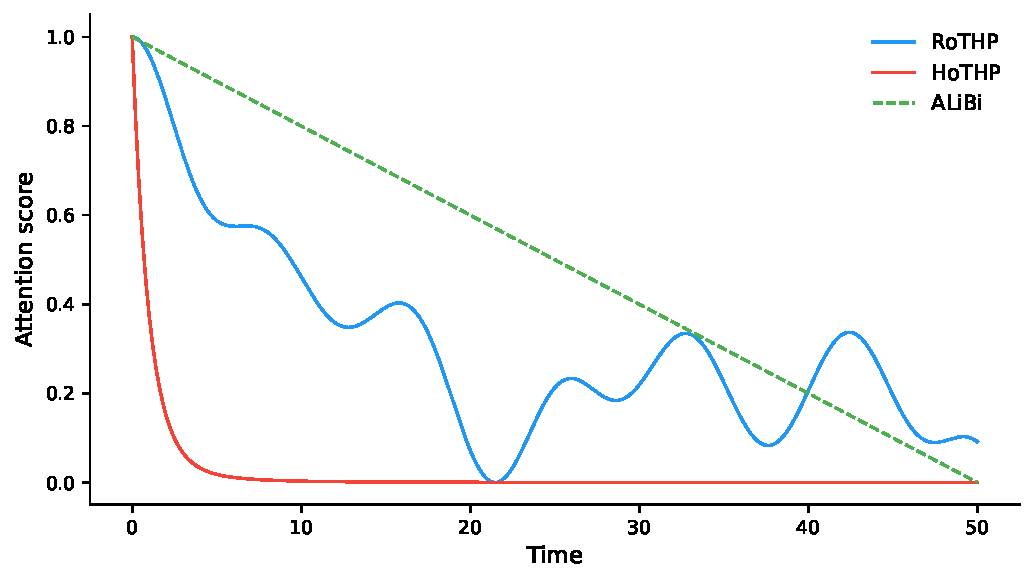
\includegraphics[width=0.75\textwidth]{figures/attention_profile.pdf}
\caption{Theoretical attention profiles as a function of $\Delta t$ for RoTHP, ALiBi, and HoTHP. The HoTHP profile most closely resembles the exponential decay kernel of the Hawkes process.}
\label{fig:attention_profile}
\end{figure}

\section{Conclusion}

In this work, we proposed HoTHP, a Transformer Hawkes Process that replaces the trigonometric rotational kernel of RoTHP with a hyperbolic kernel with learnable exponential decay, parameterized by $\theta'$. The central motivation is the structural alignment between the exponential decay induced by the hyperbolic kernel and the exponential kernel of the Hawkes process. Just as the intensity function introduced by Hawkes \cite{hawkes1971spectra} $\varphi(t) = \alpha e^{-\beta \Delta}$ imposes that past events lose influence monotonically over time, the HoTHP kernel imposes the same bias directly in the attention mechanism. This structural correspondence is not accidental but rather the inductive bias that justifies the choice of HoPE as inspiration and distinguishes HoTHP from other positional encoding approaches.

The experiments on synthetic data confirm that HoTHP generalizes better in the length extrapolation scenario (\textit{train short, test long}). In the fast decay regime, the performance difference relative to RoTHP is statistically significant (Wilcoxon $p=0.031$), with HoTHP maintaining stable NLL while RoTHP degrades progressively. In slow decay processes, HoTHP also achieves lower NLL at all extrapolation scales, although with smaller margins that do not reach statistical significance for $L=50$. Furthermore, HoTHP exhibited lower variance across different seeds and better alignment with the data-generating kernel, while maintaining the time invariance introduced by RoTHP.

The experiments were conducted exclusively on synthetic data. Although this choice allowed precise control of the generating process and isolation of the effect of positional encoding from other factors, it does not directly demonstrate performance on real data, where the dependency structure may be more complex and the generating process is unknown.

As future work, we plan to evaluate HoTHP on real-world event datasets, including financial transactions, social networks, and seismic data, where the ability to extrapolate length has a direct impact on practical applications.

\begin{credits}
\subsubsection{\ackname} 
The authors used Claude, an AI assistant by Anthropic, to support language editing and text refinement during manuscript preparation. All scientific content, experimental design, results, and conclusions were produced, reviewed, and validated entirely by the authors, who bear full responsibility for the final version of this work.

This work was supported by the National Council for Scientific and
Technological Development (CNPq), grant number 306569/2024-8.
\end{credits}

\bibliography{refs}

\end{document}
